\subsection{تخمین پارامتر کانال یاو}
برای اصلاح پارامترهای یاو چندین آزمایش انجام شد و با استفاده از داده‌های ثبت شده از وضعیت استند در کانال پیچ  و جعبه‌ابزار
\lr{Parameter Estimator}
پارامترها اصلاح شدند.
برای آزمایش یاو همه‌ی موتورها با دور مختلف شروع به حرکت کردند و از خروجی‌ سنسور داده برداری شد. سپس، مدل و پارامترهای داده‌های ثبت شده‌ی سنسور (وضعیت استند در کانال یاو) به جعبه‌ابزار
\lr{Parameter Estimator}
داده شد. نتایج آزمایش‌های کانال یاو بعد از اصلاح پارامترها در شکل
\ref{yaw_ps1} و \ref{yaw_ps2}
آورده شده است.

\begin{figure}[H]
	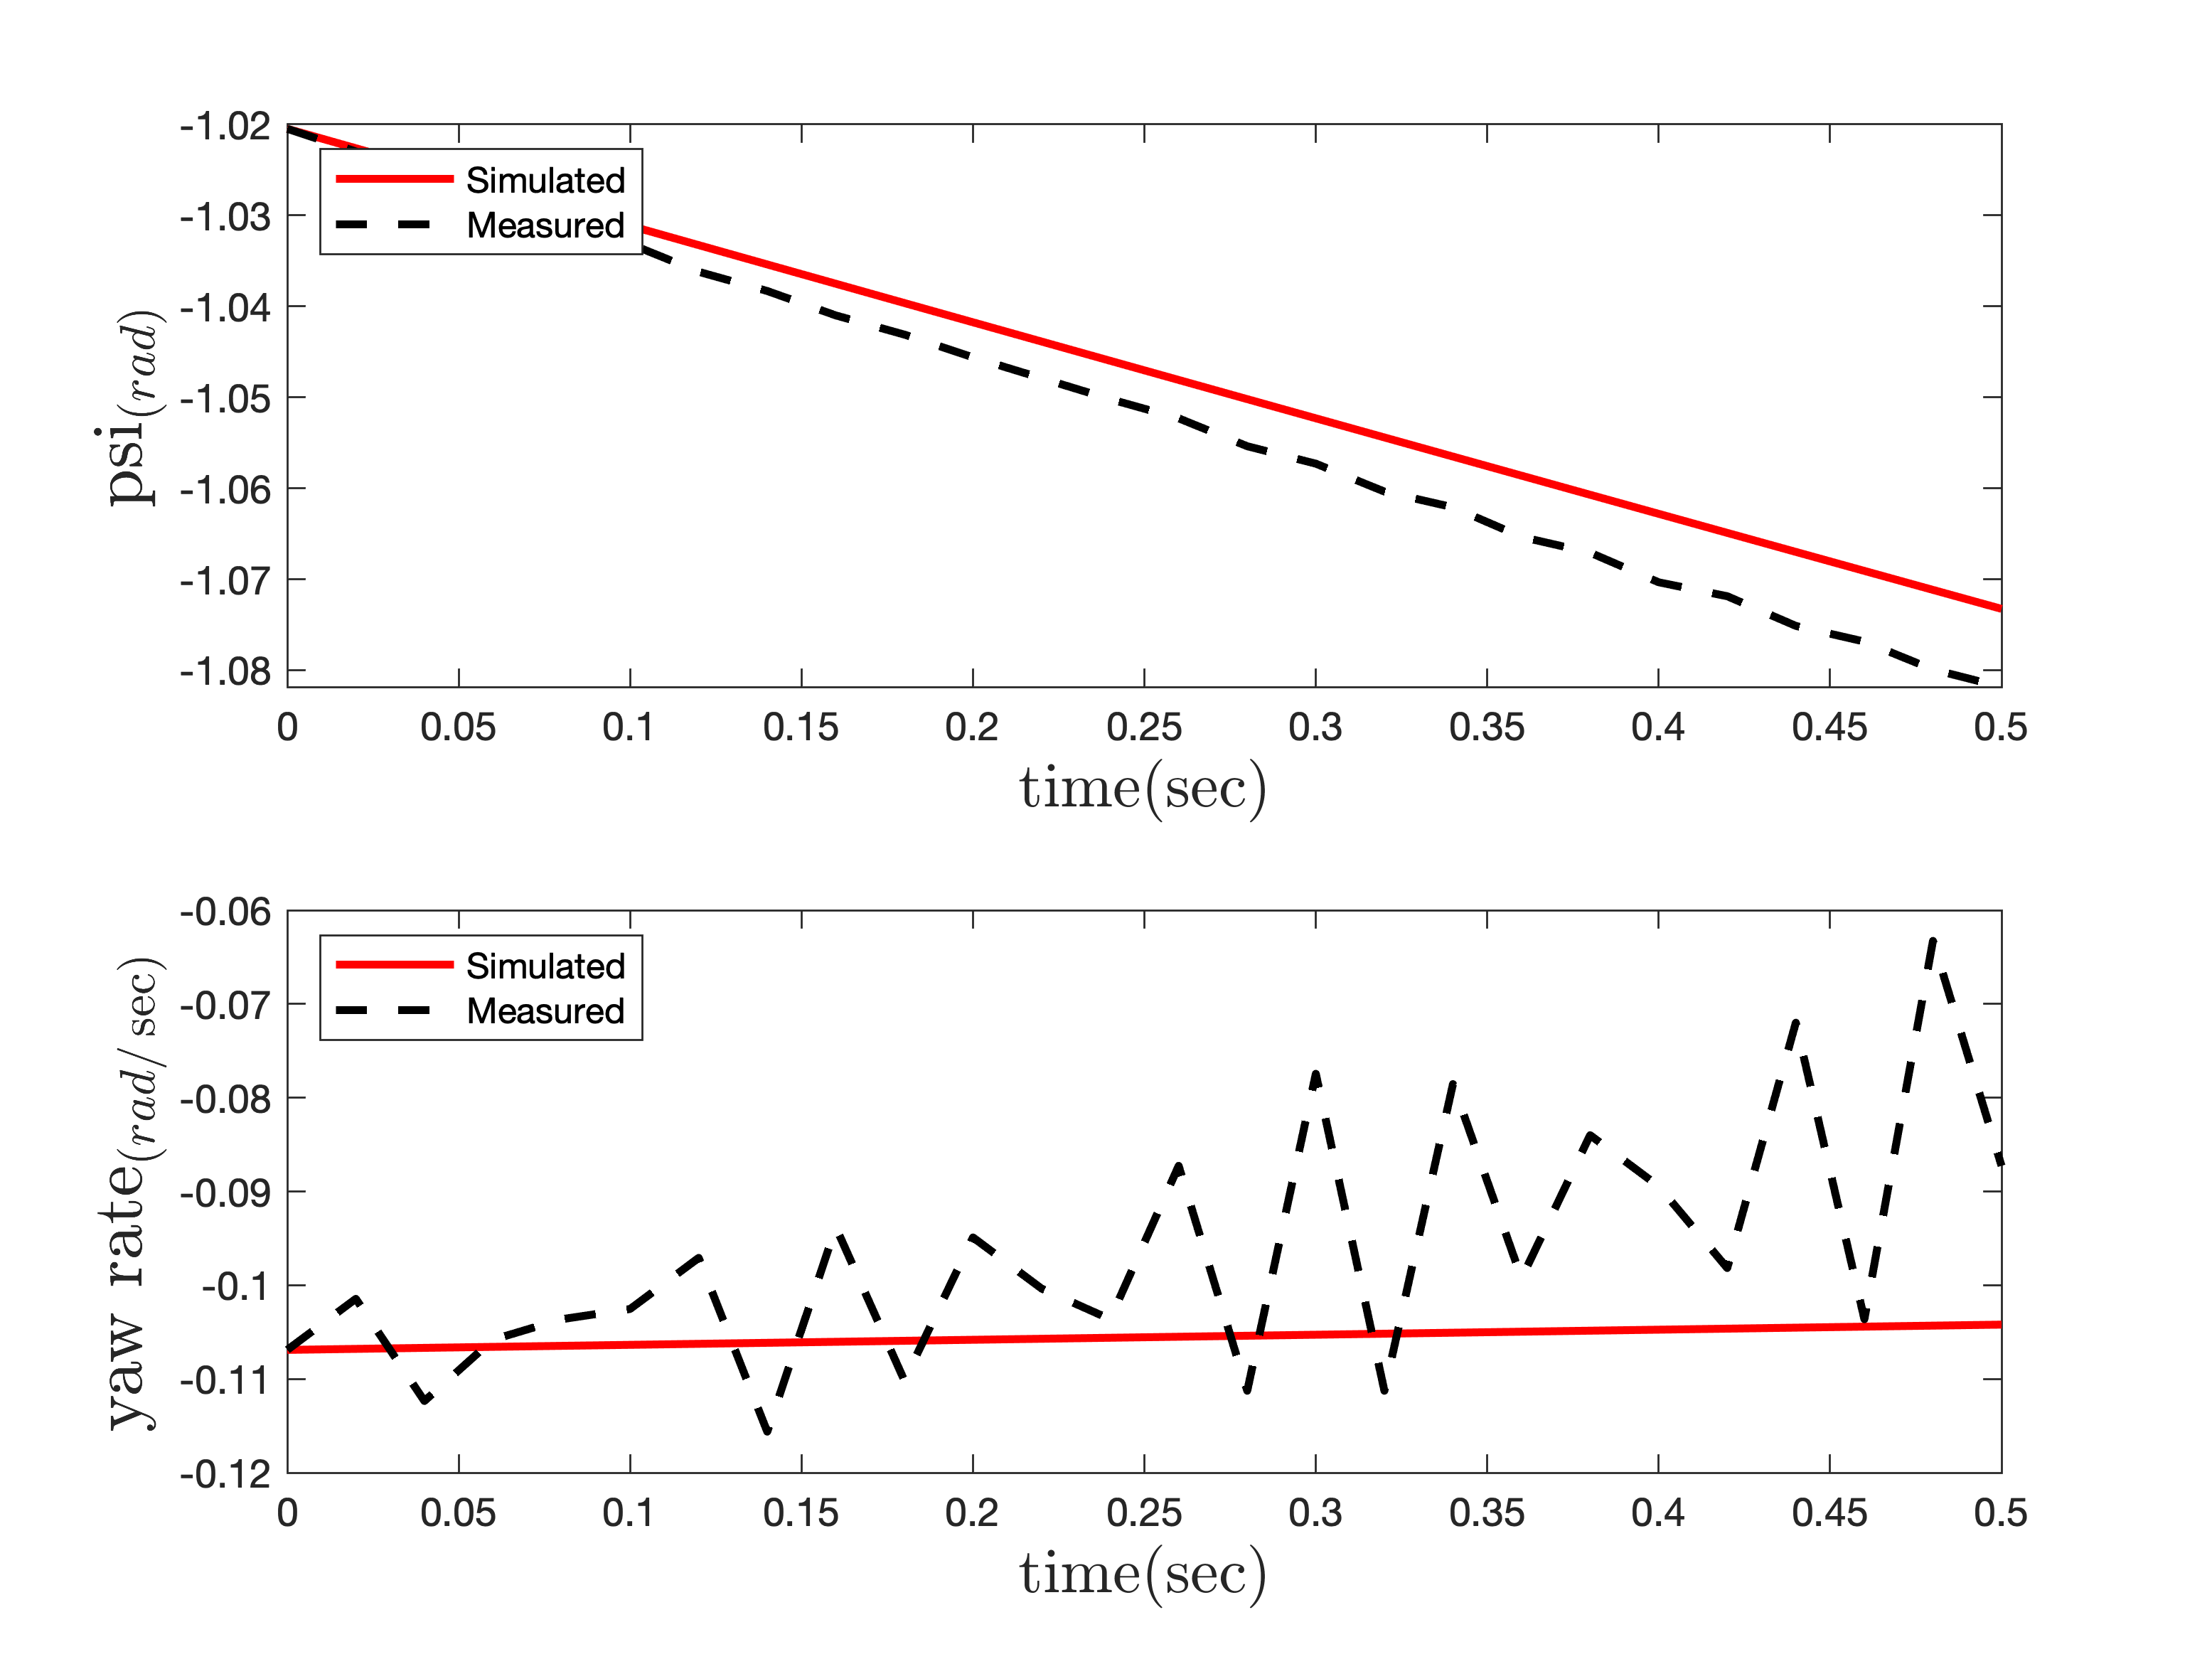
\includegraphics[width=12cm]{../Figures/RCP/yaw_parameter_estimation/RCP_yaw_S1.png}
	\centering
	\caption{مقايسه وضعیت استند در  آزمايش اول و شبیه‌سازی، پس از تخمین پارامترهای کانال یاو}
	\label{yaw_ps1}
\end{figure}

\begin{figure}[H]
	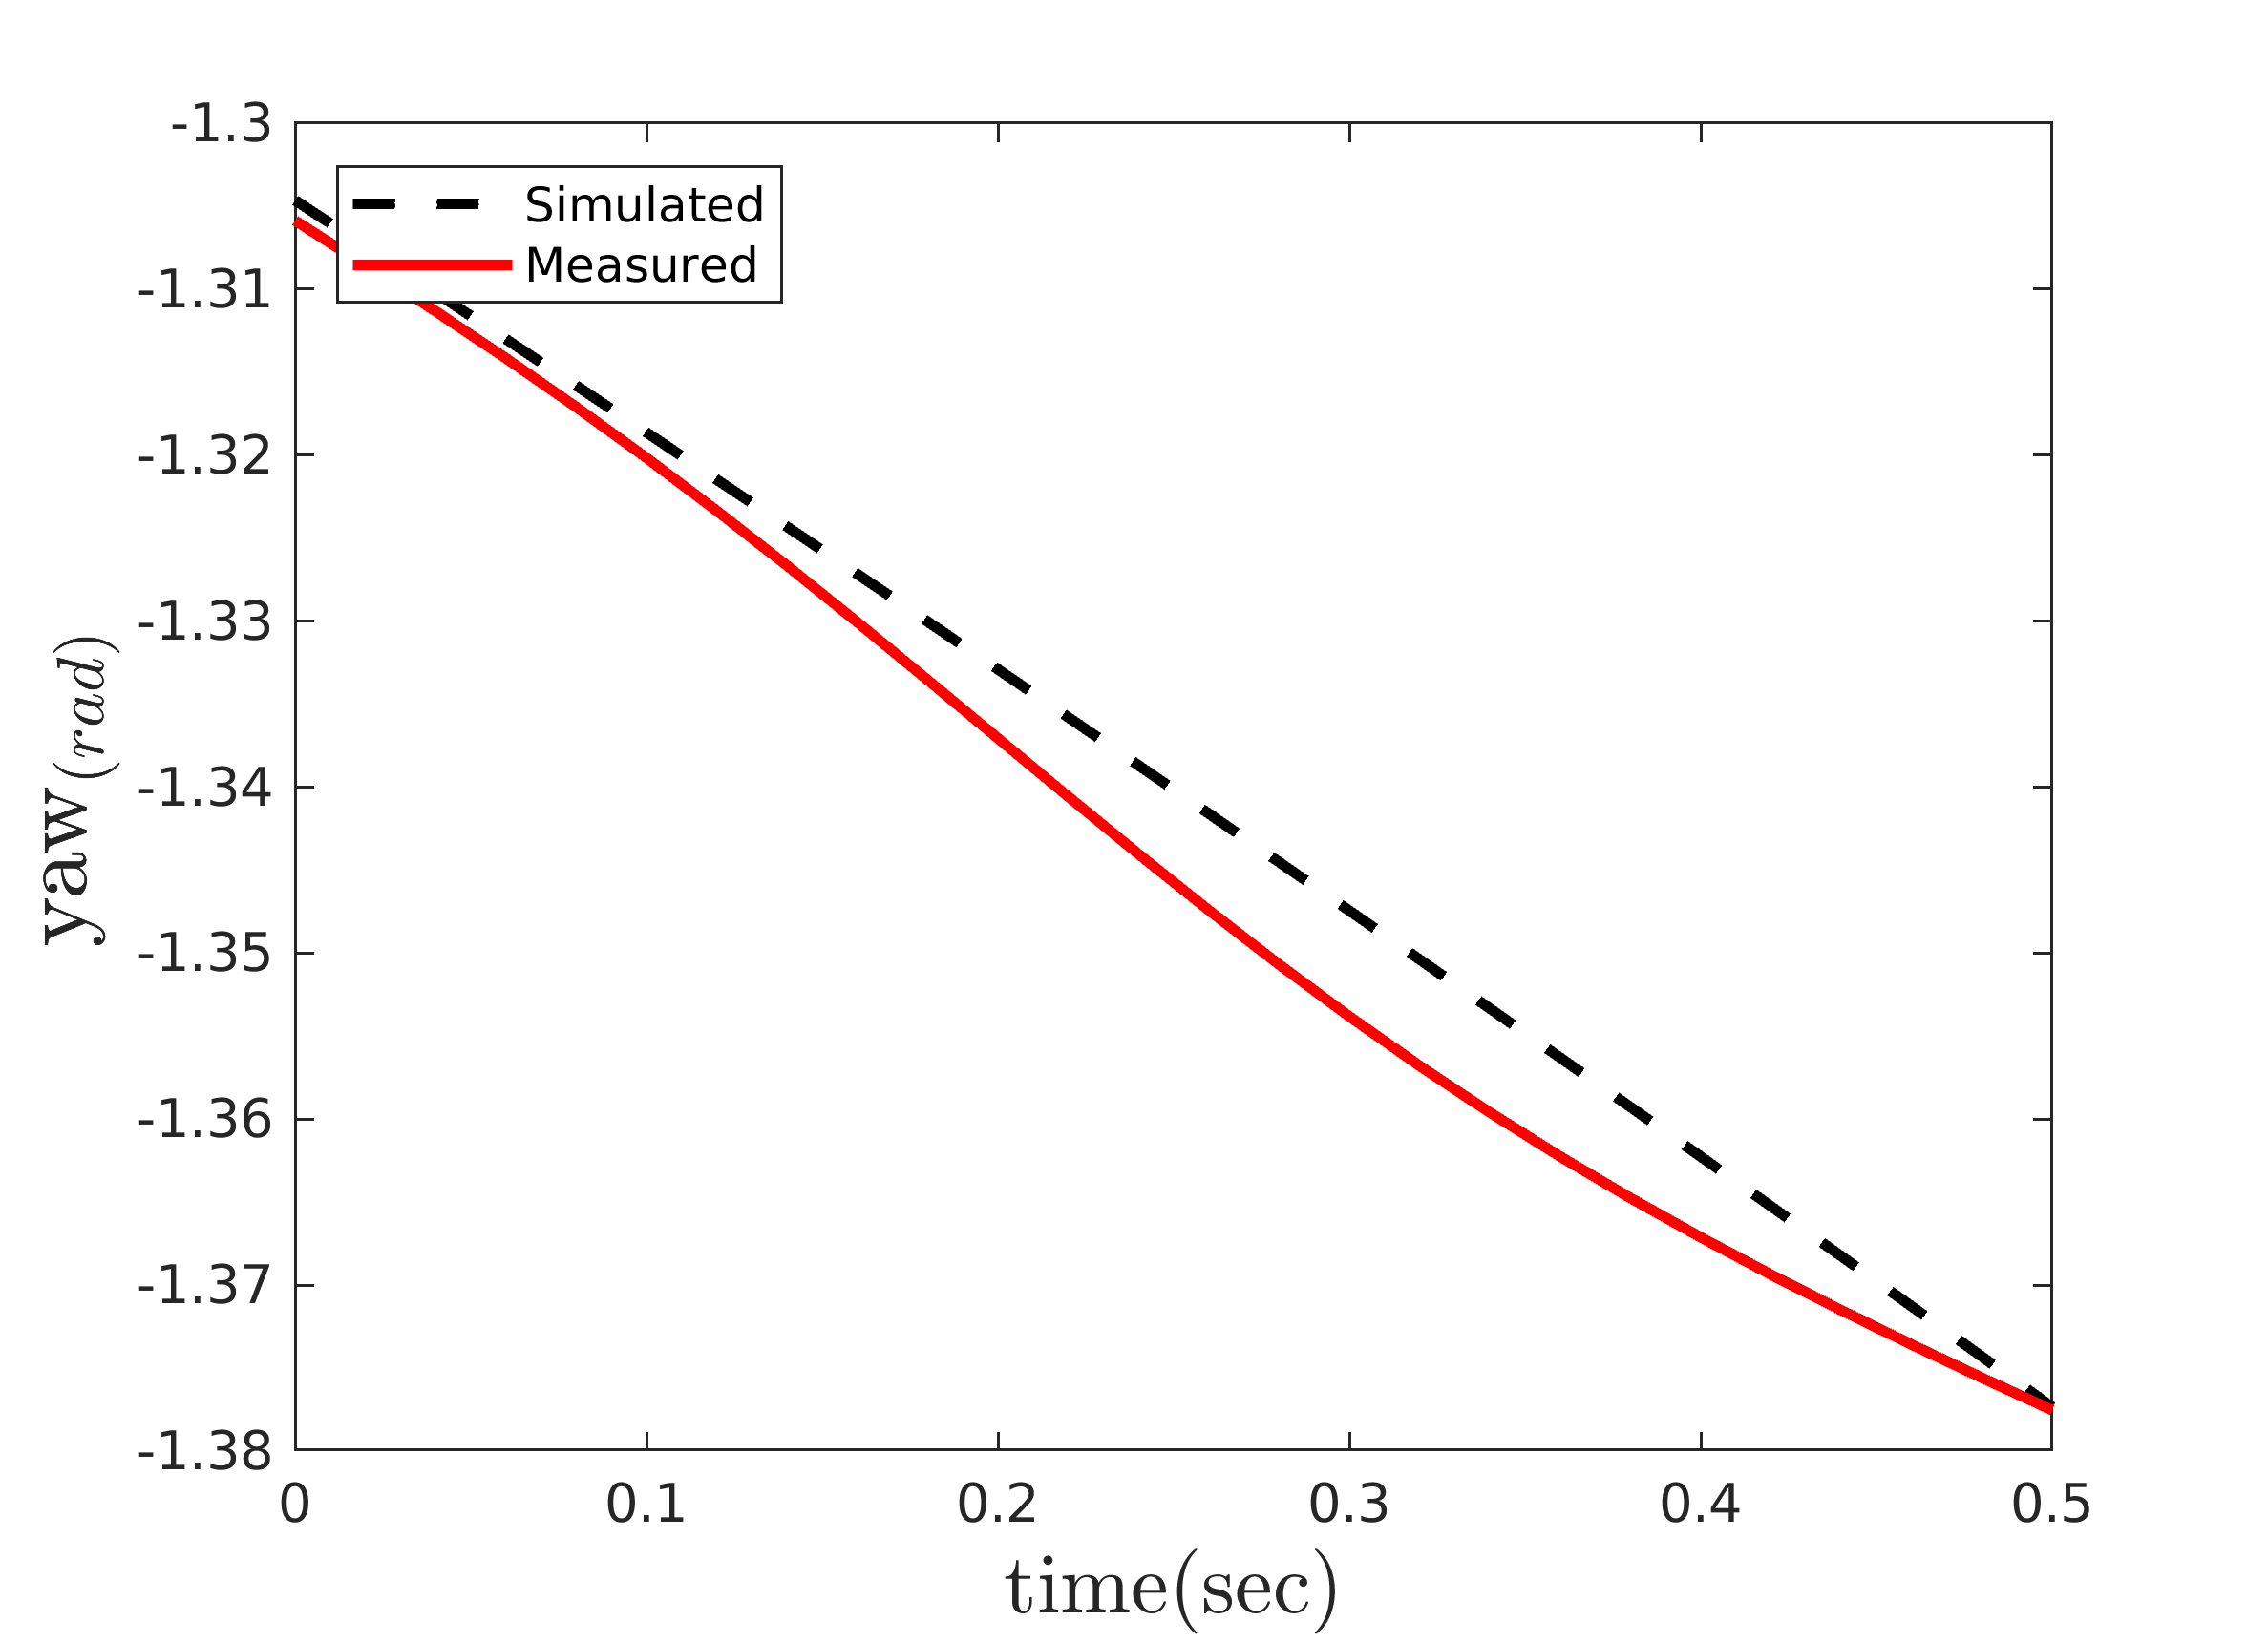
\includegraphics[width=12cm]{../Figures/RCP/yaw_parameter_estimation/RCP_yaw_S2.png}
	\centering
	\caption{مقايسه وضعیت استند در  آزمايش دوم و شبیه‌سازی، پس از تخمین پارامترهای کانال یاو}
	\label{yaw_ps2}
\end{figure}